%%%%%%%%%%%%%%%%%%%%%%%%%%%%%%%%%%%%%%%%%%%%%%%%%%%%%%%%%%%%%%%%%%%%%%
% Lớp 8 | Chương III. Tứ giác | Hình thang cân
% Dạng 8H3?11-3: Tính độ dài, số đo góc
%%%%%%%%%%%%%%%%%%%%%%%%%%%%%%%%%%%%%%%%%%%%%%%%%%%%%%%%%%%%%%%%%%%%%%


% nguồn: De_AI_Toan8_cuoi_hoc_ki_i_1 (nhập 21/11/2026)
\begin{bt}%[8H3H11-3]%[ma:da06814f]
	Cho hình thang cân $ABCD$ ($AB \parallel CD$) có $\widehat{C} = 65^\circ$. Tính số đo các góc còn lại của hình thang cân $ABCD$.
	\loigiai{
		Vì $ABCD$ là hình thang cân có hai đáy $AB \parallel CD$ nên hai góc kề một đáy bằng nhau: \\
$\widehat{D} = \widehat{C} = 65^\circ$. \\
Vì $AB \parallel CD$ nên hai góc trong cùng phía bù nhau: \\
$\widehat{A} + \widehat{D} = 180^\circ \Rightarrow \widehat{A} = 180^\circ - 65^\circ = 115^\circ$. \\
Tương tự, $\widehat{B} = \widehat{A} = 115^\circ$. \\
Vậy $\widehat{A} = \widehat{B} = 115^\circ$, $\widehat{D} = 65^\circ$.
	}
\end{bt}

% nguồn: De_AI_Toan8_cuoi_hoc_ki_i_1 (nhập 21/11/2026)
\begin{bt}%[8H3H11-3]%[ma:d58c2e0e]
	Cho hình thang cân $ABCD$ ($AB \parallel CD$) biết $\widehat{A} = 2\widehat{D}$. Tính số đo bốn góc của hình thang cân $ABCD$.
	\loigiai{
		Vì $AB \parallel CD$ nên $\widehat{A}$ và $\widehat{D}$ là hai góc trong cùng phía, suy ra $\widehat{A} + \widehat{D} = 180^\circ$. \\
Thay $\widehat{A} = 2\widehat{D}$ vào, ta được $2\widehat{D} + \widehat{D} = 180^\circ \Rightarrow 3\widehat{D} = 180^\circ \Rightarrow \widehat{D} = 60^\circ$. \\
Suy ra $\widehat{A} = 2 \cdot 60^\circ = 120^\circ$. \\
Vì $ABCD$ là hình thang cân nên $\widehat{C} = \widehat{D} = 60^\circ$ và $\widehat{B} = \widehat{A} = 120^\circ$.
	}
\end{bt}

% nguồn: De_AI_Toan8_cuoi_hoc_ki_i_1 (nhập 21/11/2026)
\begin{bt}%[8H3H11-3]%[ma:0950883b]
	Cho hình thang cân $ABCD$ ($AB \parallel CD$) có đáy nhỏ $AB = 6\text{ cm}$, đáy lớn $CD = 14\text{ cm}$ và cạnh bên $AD = 5\text{ cm}$. Kẻ các đường cao $AH$, $BK$ xuống đáy $CD$ ($H, K \in CD$).
a) Chứng minh $DH = CK$ và tính độ dài $DH$.
b) Tính độ dài đường cao $AH$ và diện tích hình thang cân $ABCD$.
	\loigiai{
		a) Xét hai tam giác vuông $AHD$ và $BKC$ ($\widehat{AHD} = \widehat{BKC} = 90^\circ$) có $AD = BC$ và $\widehat{D} = \widehat{C}$ (tính chất hình thang cân). \\
Suy ra $\triangle AHD = \triangle BKC$ (cạnh huyền – góc nhọn), nên $DH = CK$. \\
Tứ giác $ABKH$ có $AB \parallel HK$ và $AH \parallel BK$ (cùng vuông góc $CD$), lại có $\widehat{AHK} = 90^\circ$ nên $ABKH$ là hình chữ nhật, suy ra $HK = AB = 6\text{ cm}$. \\
Do đó $DH = CK = \dfrac{CD - HK}{2} = \dfrac{14 - 6}{2} = 4\text{ cm}$. \\
b) Áp dụng định lí Pythagore trong tam giác $AHD$ vuông tại $H$: $AH^2 = AD^2 - DH^2 = 5^2 - 4^2 = 9 \Rightarrow AH = 3\text{ cm}$. \\
Diện tích hình thang cân $ABCD$ là $S = \dfrac{(AB + CD) \cdot AH}{2} = \dfrac{(6 + 14) \cdot 3}{2} = 30\text{ cm}^2$.
	}
\end{bt}

% nguồn: De_AI_Toan8_cuoi_hoc_ki_i_1 (nhập 21/11/2026)
\begin{bt}%[8H3H11-3]%[ma:185765f5]
	Cho hình thang cân $ABCD$ ($AB \parallel CD$) có đáy nhỏ $AB = 8\text{ cm}$, đáy lớn $CD = 18\text{ cm}$ và đường cao $AH = 12\text{ cm}$ ($H \in CD$).
a) Tính độ dài đoạn thẳng $DH$ và cạnh bên $AD$.
b) Tính chu vi của hình thang cân $ABCD$.
	\loigiai{
		a) Kẻ thêm đường cao $BK \perp CD$ ($K \in CD$). Tương tự tính chất hình thang cân, ta có $DH = CK = \dfrac{CD - AB}{2} = \dfrac{18 - 8}{2} = 5\text{ cm}$. \\
Áp dụng định lí Pythagore trong tam giác $AHD$ vuông tại $H$: \\
$AD^2 = AH^2 + DH^2 = 12^2 + 5^2 = 144 + 25 = 169 \Rightarrow AD = 13\text{ cm}$. \\
b) Vì $ABCD$ là hình thang cân nên $BC = AD = 13\text{ cm}$. \\
Chu vi hình thang cân $ABCD$ là $AB + BC + CD + DA = 8 + 13 + 18 + 13 = 52\text{ cm}$.
	}
\end{bt}

% nguồn: De_AI_Toan8_cuoi_hoc_ki_i_1 (nhập 21/11/2026)
\begin{bt}%[8H3H11-3]%[ma:c527eb1e]
	Cho hình thang cân $ABCD$ ($AB \parallel CD$) có $AB = 5\text{ cm}$, $CD = 11\text{ cm}$ và $\widehat{D} = 60^\circ$. Kẻ đường cao $AH \perp CD$ ($H \in CD$).
a) Tính độ dài $DH$ và cạnh bên $AD$.
b) Tính chu vi của hình thang cân $ABCD$.
	\loigiai{
		a) Tương tự tính chất hai đường cao hạ từ $A$ và $B$ trong hình thang cân, ta có $DH = \dfrac{CD - AB}{2} = \dfrac{11 - 5}{2} = 3\text{ cm}$. \\
Xét tam giác $AHD$ vuông tại $H$ có $\widehat{D} = 60^\circ$, suy ra $\widehat{DAH} = 90^\circ - 60^\circ = 30^\circ$. \\
Trong tam giác vuông, cạnh góc vuông đối diện với góc $30^\circ$ bằng nửa cạnh huyền, nên $DH = \dfrac{1}{2}AD \Rightarrow AD = 2DH = 2 \cdot 3 = 6\text{ cm}$. \\
b) Vì $BC = AD = 6\text{ cm}$ nên chu vi hình thang cân $ABCD$ là $5 + 6 + 11 + 6 = 28\text{ cm}$.
	}
\end{bt}

% nguồn: chuyen_dang (nhập 22/11/2026)
\begin{bt}%[8H3H11-3]%[ma:fc07e4aa]
	Cho hình thang cân $ABCD$ với $A(2; 0)$, $B(0;  2)$, $C(0; 7)$, $D(a;b)$. Tìm giá trị nhỏ nhất của $a+b$.
	 \loigiai{
		Gọi $D(x;  y)$ suy ra $\overrightarrow{CD}=(x;y-7)$, $\overrightarrow{AD}=(x-2;y)$.\\
		$\overrightarrow{AB}=(-2;2)\Rightarrow  AB=2\sqrt{2}$, $\overrightarrow{BC}=(0;5)\Rightarrow BC=5$.
		\begin{center}
			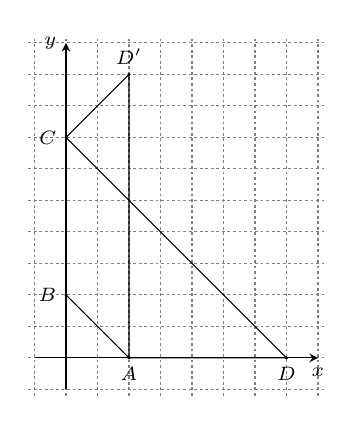
\begin{tikzpicture}[>=stealth,x=1cm,y=1cm,scale=0.4]
					 \def\a{-2}
					 \def\b{3}
					\draw[color=gray,dash pattern=on 1pt  off 1pt,xstep=1.0cm,ystep=1.0cm] (-1.2,-1.2) grid (8.2,10.2);
					\draw[->] (-1,0) -- (8,0) node[below] {\scriptsize  $x$};
					\draw[->] (0,-1) -- (0,10)  node[left] {\scriptsize $y$};
					\coordinate[label=below:\scriptsize $A$] (A) at (2,0); 
					\coordinate[label=left:\scriptsize $B$] (B)  at (0,2);
					\coordinate[label=left:\scriptsize $C$] (C) at  (0,7);
					\coordinate[label=below:\scriptsize $D$] (D) at (7,0); 
					 \coordinate[label=above:\scriptsize $D'$] (D') at (2,9);
					\draw (A)--(B)--(C)--(D)--(A) 
						 (A)--(B)--(C)--(D')--(A);
					\foreach \diem in {A,B,C,D,D'}\fill (\diem)  circle (1.5pt);
				\end{tikzpicture}
		\end{center}
		Trường hợp 1: Hình thang có hai  đáy $A B$, $C D$.\\
		Ta có $\heva{&\overrightarrow{AB},\overrightarrow{CD}\text{  cùng phương}\\&AD=BC}\Leftrightarrow\heva{&\dfrac{x}{-2}=\dfrac{y-7}{2} \\&\sqrt{(x-2)^2+y^2}=5} \Leftrightarrow\heva{&x=-y+7 \\&(-y+7-2)^2+y^2=25}$\\
		$\Leftrightarrow\heva{&x=-y+7 \\&2 y^2-10 y+25=25} \Leftrightarrow\heva{&x=7 \\&y=0} \ \text{hoặc}\ \heva{&x=2 \\&y=5.}$\\ 
		Với $\heva{&x=7 \\&y=0}$ thì  $CD=\sqrt{7^2+(0-7)^2}=7 \sqrt{2} \neq AB$ nên $D(7; 0)$ thỏa mãn.\\
		Với $\heva{&x=2 \\&y=5}$ thì $CD=\sqrt{2^2+(5-7)^2}=2 \sqrt{2}=AB$  (loại).\\
		Trường  hợp 2: Hình thang có hai đáy $BC$, $AD$.\\
		Ta có  $\heva{&\overrightarrow{BC},\overrightarrow{AD}\text{ cùng phương}\\&AB=CD}\Leftrightarrow\heva{&\dfrac{0}{x-2}=\dfrac{5}{y} \\&2\sqrt{2}=\sqrt{x^2+(y-7)^2}} \Leftrightarrow\heva{&\dfrac{x-2}{y}=\dfrac{0}{5} \\&x^2+(y-7)^2=8}$\\
		$\Leftrightarrow\heva{&x=2 \\&(y-7)^2=4} \Leftrightarrow\heva{&x=2 \\&y=5} \ \text{hoặc}\  \heva{&x=2 \\&y=9.}$\\
		 Với $\heva{&x=2 \\&y=9}$ thì $AD=\sqrt{0^2+9^2}=9 \neq BC$ nên $D(2;9)$ thỏa mãn.\\
		Với $\heva{&x=2  \\&y=5}$ thì $AD=\sqrt{0^2+5^2}=5=BC$ (loại).\\
		Vậy giá trị nhỏ nhất của  $a+b$ là $7$.
	 }
\end{bt}
